\begin{ex}
	Điền các từ thích hợp vào chỗ trống được đánh số trong đoạn văn sau. Các từ cần điền được liệt kê trong bảng bên dưới (không sử dụng lại từ đã dùng).
	
	Ở cùng điều kiện áp suất không đổi, các phân tử của chất ở thể rắn dao động nhiệt ổn định xung quanh các vị trí \textbf{(1)} tạo thành các mạng \textbf{(2)} giữ cho hình dạng riêng của chất ổn định.
	
	Khi được cung cấp \textbf{(3)} nhiệt độ của chất \textbf{(4)} và chuyển động nhiệt của các phân tử trở nên hỗn loạn hơn, khiến các nút mạng liên kết bị \textbf{(5)}. Chất bắt đầu chuyển dần sang \textbf{(6)} có thể tích riêng nhưng \textbf{(7)} không xác định.
	
\begin{center}
	\renewcommand{\arraystretch}{1.3}
	\begin{tabular}{|c|c|c|c|c|c|c|}
		\hline
		\textbf{} & \textbf{} & \textbf{} & \textbf{} & \textbf{} & \textbf{} & \textbf{} \\
		\hline
		cân bằng & liên kết & nhiệt lượng & tăng & phá vỡ & thể lỏng & hình dạng \\
		\hline
	\end{tabular}
\end{center}

	
	\loigiai{
		\begin{itemize}
			\item (1) cân bằng,\quad (2) liên kết,\quad (3) nhiệt lượng,\quad (4) tăng,\\
			\item (5) phá vỡ,\quad (6) thể lỏng,\quad (7) hình dạng.
		\end{itemize}
	}
\end{ex}
\begin{ex}
	Cho đồ thị biểu diễn quá trình chuyển thể của một chất như hình dưới đây.
	\begin{center}
		\begin{tikzpicture}[scale=1,draw=Mapcolor, very thick, >=stealth']
			\tkzDefPoints{0/0/o,8.5/0/x, 0/5/y}
			\tkzDrawSegments[very thick,Mapcolor,->](o,x o,y)
			\tkzLabelPoint[below left](o){$0$}
			\node[rotate=90] at (-0.5,2.5) {Nhiệt độ ($^\circ C$)};
			\node at (4,-0.5) {Thời gian};
			\draw (1,1) -- (1,0.5) -- (2.5,0.5) -- (2.5,1) -- (1,1);
			\draw (1.5,1.6) -- (3,1.6) -- (3,2.1) -- (1.5,2.1) -- (1.5,1.6);
			\draw (4,2.5) -- (4,2) -- (5.5,2) -- (5.5,2.5) -- (4,2.5);
			\draw (4.5,3.1) -- (6,3.1) -- (6,3.6) -- (4.5,3.6) -- (4.5,3.1);
			\draw (7,4) -- (7,3.5) -- (8.5,3.5) -- (8.5,4) -- (7,4);
			\draw[red,very thick] (0,0) -- (1.5,1.5) -- (3,1.5) -- (4.5,3) -- (6,3) -- (7.5,4.5);
			
			\node at (0.8,1.2) {1)};
			\node at (3.8,2.7) {2)};
			\node at (6.8,4.2) {3)};
		\end{tikzpicture}
	\end{center}
	\begin{enumerate}[label=\alph*)]
		\item Điền nội dung thích hợp vào các ô trống trong hình.
		\item Trên trục nhiệt độ chỉ ra nhiệt độ nóng chảy và nhiệt độ sôi của chất đang xét.
		\item Dựa vào mô hình động học phân tử, hãy giải thích điều gì đang xảy ra tại các đoạn 1), 2) và 3) trên đồ thị.
		
	\end{enumerate}
	\loigiai{
		\begin{itemize}
			\item Điền nội dung thích hợp vào các ô trống trong Hình 1.7.
			\begin{description}
				\item[1)]: Chất rắn nóng chảy
				\item[2)]: Chất lỏng
				\item[3)]: Chất lỏng sôi và chuyển sang hơi
			\end{description}
			\item Trên trục nhiệt độ chỉ ra nhiệt độ nóng chảy và nhiệt độ sôi của chất đang xét.
			\begin{description}
				\item[Nhiệt độ nóng chảy] $T_{\text{nóng chảy}}$
				\item[Nhiệt độ sôi] $T_\text{sôi}$
			\end{description}
			\item Dựa vào mô hình động học phân tử, hãy giải thích điều gì đang xảy ra tại các đoạn 1), 2) và 3) trên đồ thị.
			\begin{description}
				\item[1)]: Tại đoạn này, chất rắn đang nhận nhiệt và nhiệt độ tăng dần cho đến khi đạt đến nhiệt độ nóng chảy và chuyển thành chất lỏng. 
				\item[2)]: Tại đoạn này, chất lỏng tiếp tục nhận nhiệt lượng nhưng nhiệt độ không đổi vì nhiệt lượng dùng để phá vỡ lực liên kết giữa các phân tử, chuyển từ lỏng sang hơi.
				\item[3)]: Tại đoạn này, chất lỏng đã sôi và chuyển hoàn toàn thành hơi, tiếp tục nhận nhiệt và tăng nhiệt độ của hơi.
			\end{description}
			
		\end{itemize}
	}
\end{ex}

\loai{Khái niệm nhiệt nóng chảy riêng}
\begin{ex}
	Phát biểu nào sau đây là đúng khi nói về nhiệt nóng chảy riêng?
	\choice
	{Nhiệt nóng chảy riêng của một chất có độ lớn bằng nhiệt lượng cần cung cấp để làm nóng chảy 1 kg chất đó ở nhiệt độ nóng chảy}
	{Đơn vị của nhiệt nóng chảy riêng là Jun trên kilôgam (J/kg)}
	{Các chất khác nhau thì nhiệt nóng chảy riêng của chúng khác nhau}
	{\True Cả A, B, C đều đúng}
	\loigiai{
		
		- "Nhiệt nóng chảy riêng của một chất có độ lớn bằng nhiệt lượng cần cung cấp để làm nóng chảy 1 kg chất đó ở nhiệt độ nóng chảy" là đúng. Đây là định nghĩa của nhiệt nóng chảy riêng ($\lambda$).
		
		- "Đơn vị của nhiệt nóng chảy riêng là Jun trên kilôgam (J/kg)" là đúng. Nhiệt nóng chảy riêng được tính bằng năng lượng trên khối lượng.
		
		- "Các chất khác nhau thì nhiệt nóng chảy riêng của chúng khác nhau" là đúng. Nhiệt nóng chảy riêng đặc trưng cho từng chất và thay đổi tùy theo chất đó.
		
		Vì vậy, phát biểu "Cả A, B, C đều đúng" là đúng.
	}
	\haidong{2}
\end{ex}
\loai{Đặc điểm của nhiệt nóng chảy riêng}
\begin{ex}%[1P7B4-1][Loai1]
	Nhiệt nóng chảy riêng của vật rắn phụ thuộc vào
	\choice
	{nhiệt độ của vật rắn và áp suất ngoài}
	{\True bản chất của vật rắn}
	{bản chất và nhiệt độ của vật rắn}
	{bản chất và nhiệt độ của vật rắn, đồng thời phụ thuộc áp suất ngoài}
	\loigiai{
		Nhiệt nóng chảy riêng $\lambda$ phụ thuộc bản chất vật rắn.
	}%<MyLT2>
	\haidong{2}\end{ex}
	\loai{Ý nghĩa của nhiệt nóng chảy riêng}
	\begin{ex}
		Nhiệt nóng chảy riêng của đồng là $1,8 . 10^{5} \ J / kg$ có nghĩa là
		\choice
		{khối đồng sẽ toả ra nhiệt lượng $1,8 . 10^{5} \ J$ khi nóng chảy hoàn toàn}
		{\True mỗi kilôgam đồng cần thu nhiệt lượng $1,8 . 10^{5} \ J$ để hoá lỏng hoàn toàn ở nhiệt độ nóng chảy}
		{khối đồng cần thu nhiệt lượng $1,8 . 10^{5} \ J$ để hoá lỏng}
		{mỗi kilôgam đồng toả ra nhiệt lượng $1,8 . 10^{5} \ J$ khi hoá lỏng hoàn toàn}
		\loigiai{        
			Nhiệt nóng chảy riêng của một chất, ký hiệu là $\lambda$, biểu thị nhiệt lượng cần cung cấp cho 1 kg chất đó để nó chuyển từ pha rắn sang pha lỏng hoàn toàn ở nhiệt độ nóng chảy của nó mà không thay đổi nhiệt độ. Đơn vị của nhiệt nóng chảy riêng là $\dfrac{J}{kg}$.
			
			\[
			\lambda_{\text{đồng}} = 1,8 . 10^{5} \ \dfrac{J}{kg}
			\]
			
			Điều này có nghĩa là mỗi kilôgam đồng cần thu nhiệt lượng $1,8 . 10^{5} \ J$ để hoá lỏng hoàn toàn ở nhiệt độ nóng chảy. Các đáp án khác không đúng vì:
			
			- "Khối đồng sẽ toả ra nhiệt lượng $1,8 . 10^{5} \ J$ khi nóng chảy hoàn toàn" là sai vì nhiệt nóng chảy là lượng nhiệt cần cung cấp, không phải nhiệt toả ra.
			
			- "Khối đồng cần thu nhiệt lượng $1,8 . 10^{5} \ J$ để hoá lỏng" không chính xác vì không đề cập rõ khối lượng bao nhiêu.
			
			- "Mỗi kilôgam đồng toả ra nhiệt lượng $1,8 . 10^{5} \ J$ khi hoá lỏng hoàn toàn" là sai, chất khi hóa lỏng cần thu nhiệt, không phải tỏa nhiệt.
		}
		\haidong{2}
	\end{ex}
	\loai{Đặc điểm của quá trình nóng chảy}
	\begin{ex}
		Khi vật rắn tinh thể đang nóng chảy thì đại lượng nào của vật \textbf{không} thay đổi?
		\choice
		{Thể tích của vật}
		{Nội năng của vật}
		{\True Nhiệt độ của vật}
		{Hình dạng của vật}
		\loigiai{
			\item Trong quá trình nóng chảy của vật rắn tinh thể, nhiệt độ của vật không thay đổi. \item Điều này có nghĩa là nhiệt độ của vật duy trì ở nhiệt độ nóng chảy suốt quá trình nóng chảy. \item Lượng nhiệt cung cấp cho vật sử dụng để phá vỡ cấu trúc tinh thể, chuyển vật từ pha rắn sang pha lỏng mà không làm tăng nhiệt độ. 
			
			\item Các đại lượng khác như thể tích và nội năng có thể thay đổi. \item Thể tích của vật có thể thay đổi do sự nở ra khi chuyển từ rắn sang lỏng, trong khi nội năng tăng do nhiệt lượng hấp thụ.
		}
		\haidong{2}
	\end{ex}
	\loai{Thí nghiệm đo nhiệt nóng chảy riêng}
	\begin{ex} \nguon{2}
		Các thao tác cơ bản để đo nhiệt nóng chảy riêng của cục nước đá với các dụng cụ như hình dưới
		\begin{center}
			\begin{tikzpicture}[scale=1,thick,>=stealth']
				\node[rotate=0] (russell) at (-1,0.5) {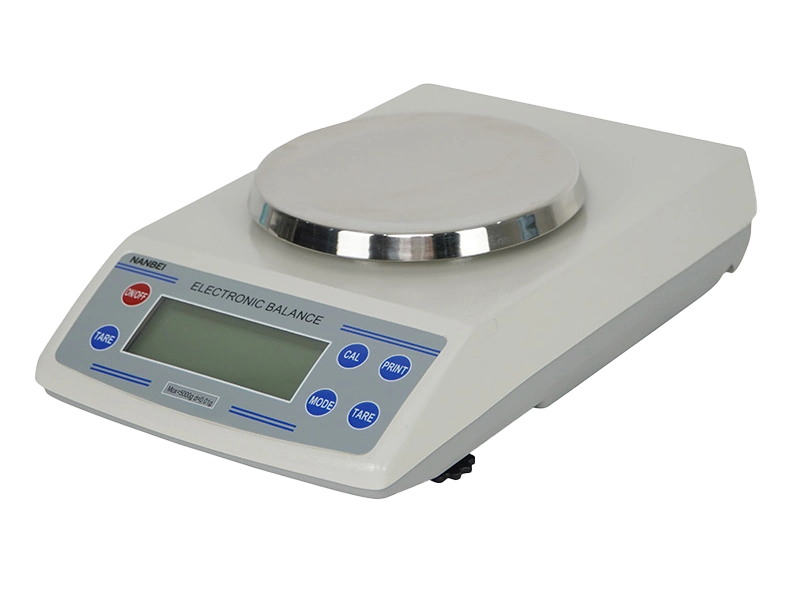
\includegraphics[width=2.2cm]{Images/candientu}};
				\node[rotate=0] (russell) at (1.5,0.5) {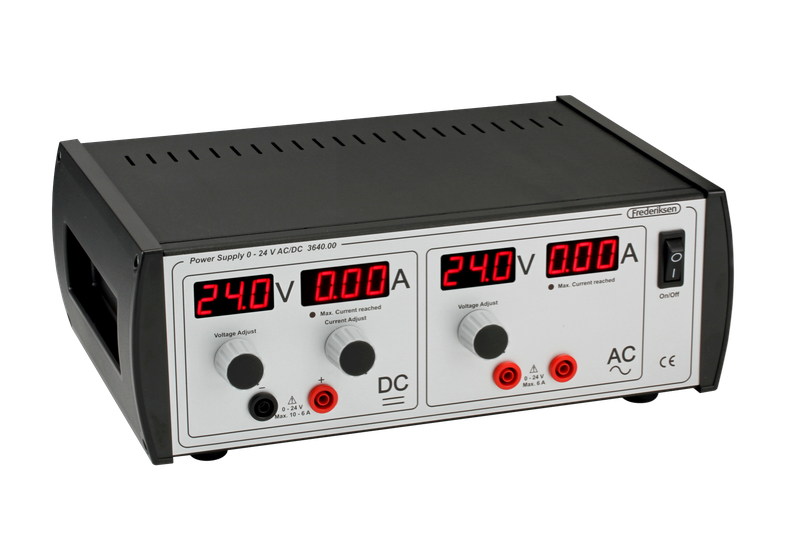
\includegraphics[width=2.8cm]{Images/bienthenguon}};
				\node[rotate=0] (russell) at (4,0.5) {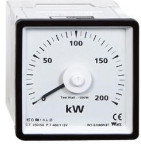
\includegraphics[width=1.5cm]{Images/oatke}};
				\node[rotate=0] (russell) at (6.5,1) {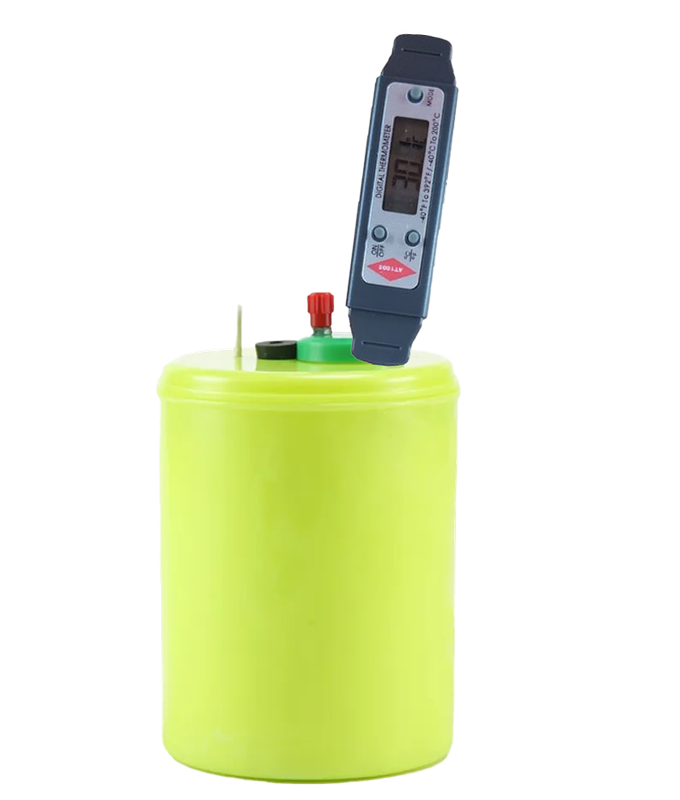
\includegraphics[width=2.6cm]{Images/nlkvank}};
				
				\node at (-1,2.5) {(5)};
				\node at (0.8,2.45) {(1)};
				\node at (4.5,-1) {(2)};
				\node at (7.5,-1.5) {(4)};
				\draw (-1,2) -- (-1,1);
				\draw (1,2) -- (1.5,1);
				\draw (4.35,-0.75) -- (4,-0.3);
				\draw (6.45,-0.65) -- (7.2,-1.25);
				\draw (6.5,2) -- (5.5,2.5);
				\node at (5.15,2.7) {(3)};
			\end{tikzpicture}
		\end{center}
		\begin{itemize} 
			\item [a.] Khuấy liên tục nước đá, cứ sau 2 phút lại đọc số đo trên oát kế và nhiệt độ trên nhiệt kế rồi ghi lại kết quả. 
			\item [b.] Cho viên nước đá khối lượng $m\ kg$ và một ít nước lạnh vào bình nhiệt lượng kế, sao cho toàn bộ điện trở chìm trong hỗn hợp nước đá. 
			\item [c.] Bật nguồn điện.
			\item [d.] Cắm đầu đo của nhiệt kế vào bình nhiệt lượng kế.
			\item [e.] Nối oát kế với nhiệt lượng kế và nguồn điện.
		\end{itemize} 
		Thứ tự đúng các thao tác là
		\choice
		{$b,\ a,\ c,\ d,\ e$}
		{\True $b,\ d,\ e,\ c,\ a$}
		{$b,\ d,\ a,\ e,\ c$}
		{$b,\ d,\ a,\ c,\ e$}
		\loigiai{
			Thứ tự đúng để đo nhiệt nóng chảy riêng của cục nước đá là: b, d, e, c, a.
		}
	\end{ex}
	\begin{ex}
		Đồ thị nào sau đây biểu diễn sự thay đổi nhiệt độ theo thời gian của nước ở $25^\circ C$ trong bình nhiệt lượng kế?
		\begin{center}
			\begin{tikzpicture}[scale=0.9,draw=Mapcolor, very thick, >=stealth']
				\tkzDefPoints{0/0/o, 3/0/x, 0/3/y}
				\tkzDrawSegments[->](o,x o,y)
				\tkzLabelPoint[left](o){$O$}
				\tkzLabelPoint[above](x){$\tau\ (s)$}
				\tkzLabelPoint[above](y){$t\ (^\circ C)$}
				\node[left] at (0,1) {$25$};
				\node at (1.5,-0.5) {(1)};
				\draw[blue,very thick] (0,1) -- (2.25,0.25);
				
				\begin{scope}[shift={(5,0)},rotate=0]
					\tkzDefPoints{0/0/o, 3/0/x, 0/3/y}
					\tkzDrawSegments[->](o,x o,y)
					\tkzLabelPoint[left](o){$O$}
					\tkzLabelPoint[above](x){$\tau\ (s)$}
					\tkzLabelPoint[above](y){$t\ (^\circ C)$}
					\node[left] at (0,1) {$25$};
					\node at (1.5,-0.5) {(2)};
					\draw[blue, very thick] (0,1) .. controls (1,1.25) and (1.75,1.5) .. (2.5,2.5);
				\end{scope}
				
				\begin{scope}[shift={(10,0)},rotate=0]
					\tkzDefPoints{0/0/o, 3/0/x, 0/3/y}
					\tkzDrawSegments[->](o,x o,y)
					\tkzLabelPoint[left](o){$O$}
					\tkzLabelPoint[above](x){$\tau\ (s)$}
					\tkzLabelPoint[above](y){$t\ (^\circ C)$}
					\node[left] at (0,1) {$25$};
					\node at (1.5,-0.5) {(3)};
					\draw[blue,very thick] (0,1) -- (2.75,2.5);
				\end{scope}
				
				\begin{scope}[shift={(15,0)},rotate=0]
					\tkzDefPoints{0/0/o, 3/0/x, 0/3/y}
					\tkzDrawSegments[->](o,x o,y)
					\tkzLabelPoint[left](o){$O$}
					\tkzLabelPoint[above](x){$\tau\ (s)$}
					\tkzLabelPoint[above](y){$t\ (^\circ C)$}
					\node[left] at (0,1) {$25$};
					\node at (1.5,-0.5) {(4)};
					\draw[blue, very thick] (0,1) .. controls (0.75,0.5) and (1.75,0.25) .. (2.25,0.25);
				\end{scope}
				
				
			\end{tikzpicture}
		\end{center}
		
		\choice
		{Đồ thị (1)}
		{Đồ thị (2)}
		{\True Đồ thị (3)}
		{Đồ thị (4)}
		\loigiai{Đồ thị 3
		}
		\haidong{2}\end{ex}
\begin{ex} \nguon{2}
	\immini[thm]{Đồ thị biểu diễn sự phụ thuộc của nhiệt độ $t$ vào nhiệt lượng $Q$ mà chất hấp thụ. Khối lượng của chất là $2 \ kg$. Ban đầu, chất này ở trạng thái rắn. Nhiệt nóng chảy riêng của chất này là
		\choice
		{\True $2 . 10^{5} \ J /kg$}
		{$3 . 10^{5} \ J /kg$}
		{$2,5 . 10^{5} \ J /kg$}
		{$2,01 . 10^{5} \ J /kg$}}{\begin{tikzpicture}[draw=Mapcolor, very thick, ]
 %Hệ trục toạ độ
 \tkzDefPoints{0/0/x', 6/0/x, 0/0/y', 0/4/y}
 \tkzDrawSegments[very thick, Mapcolor,->](x',x y',y)
 \tkzLabelPoint[below](x){$Q.10^5\ (J)$}
  \tkzLabelPoint[above](y){$t\ (^\circ C)$}
 \draw  [help  lines, xstep=0.5cm,ystep=0.5cm]  (x' |- y')  grid  (x |- y);
\foreach  \x  in  {0,1,...,4}
{\draw[thin]  (\x,-0.1)  --  (\x,0.1);}
\foreach  \x  in  {1,2,...,5}
{\pgfmathtruncatemacro{\label}{2*\x};
	\node[below]
	(\label) at (\x,0) {\label};}
\node[below left] at (0,0){$O$};
\draw[red, very thick](0,0.5)--(2,2)--(4,2)--(5.5,3.75);
\end{tikzpicture}}
	\loigiai{
		\begin{itemize}
			\item Khi nóng chảy chất nhận được nhiệt lượng $4 . 10^{5} \ J$
			\item Nhiệt nóng chảy riêng được tính như sau:
			\begin{align*}
				\lambda=\dfrac{Q}{m}=\dfrac{4 . 10^{5}}{2}=2 . 10^{5} \ J / kg
			\end{align*}
		\end{itemize}
	}
\end{ex}
\loai{Định nghĩa nhiệt hóa hơi riêng}
\begin{ex} \nguon{4}
	Nhiệt hóa hơi riêng của một chất lỏng là nhiệt lượng cần thiết để
	\choice
	{\True làm cho một kilôgam chất lỏng đó hóa hơi hoàn toàn ở nhiệt độ xác định}
	{làm cho một kilôgam chất lỏng tăng thêm $1^\circ C$}
	{làm cho một khối lượng xác định chất lỏng đó hóa hơi hoàn toàn}
	{làm cho một kilôgam hơi chuyển hoàn toàn sang thể lỏng ở nhiệt độ xác định}
	
	\loigiai{
		Nhiệt hóa hơi riêng là nhiệt lượng cần thiết để làm hóa hơi hoàn toàn 1 kg chất lỏng tại nhiệt độ xác định.
	}
\end{ex}
\loai{Đơn vị của nhiệt hóa hơi riêng}
\begin{ex}
	Đơn vị của nhiệt hóa hơi riêng là
	\choice
	{\True $J / kg$}
	{J.kg}
	{$kg / J$}
	{J}
	\loigiai{
		\item Nhiệt hóa hơi riêng biểu thị nhiệt lượng cần cung cấp để hóa hơi hoàn toàn một kg chất lỏng ở nhiệt độ hóa hơi của nó. 
		\item Do đó, đơn vị của nhiệt hóa hơi riêng là năng lượng trên khối lượng, được đo bằng Jun trên kilôgam (J/kg).
	}
	\haidong{2}
\end{ex}
\loai{Ý nghĩa của nhiệt hóa hơi riêng}
\begin{ex}
	Nhiệt hóa hơi riêng của nước là $2,3 . 10^6\ J/kg$ ở nhiệt độ $100^\circ C$ có nghĩa là
	\choice
	{một lượng nước bất kì cần thu một lượng nhiệt là $2,3 . 10^6 \ J$ để bay hơi hoàn toàn}
	{mỗi kilogam nước cần thu một lượng nhiệt là $2,3 . 10^6 \ J$ để bay hơi hoàn toàn}
	{mỗi kilogam nước sẽ tỏa ra một lượng nhiệt là $2,3 . 10^6 \ J$ khi bay hơi hoàn toàn ở nhiệt độ $100^\circ C$}
	{\True mỗi kilogam nước cần thu một lượng nhiệt là $2,3 . 10^6 \ J$ để bay hơi hoàn toàn ở nhiệt độ $100^\circ C$}
	\loigiai{
		\item Nhiệt hóa hơi riêng của nước là giá trị nhiệt lượng cần cung cấp để một kilogam nước bay hơi hoàn toàn ở nhiệt độ sôi ($100^\circ C$) và áp suất tiêu chuẩn (1 atm).
		
		\item  "Một lượng nước bất kì cần thu một lượng nhiệt là $2,3 . 10^6 \ J$ để bay hơi hoàn toàn" không đúng vì nhiệt hóa hơi riêng là nhiệt hóa hơi tính cho 1 đơn vị khối lượng.
		
		\item  "Mỗi kilogam nước cần thu một lượng nhiệt là $2,3 . 10^6 \ J$ để bay hơi hoàn toàn" đúng nhưng thiếu điều kiện cần thiết về nhiệt độ và áp suất.
		
		\item  "Mỗi kilogam nước sẽ tỏa ra một lượng nhiệt là $2,3 . 10^6 \ J$ khi bay hơi hoàn toàn ở nhiệt độ sôi" là sai, vì nước cần thu nhiệt để bay hơi, không tỏa nhiệt.
		
		\item  "Mỗi kilogam nước cần thu một lượng nhiệt là $2,3 . 10^6 \ J$ để bay hơi hoàn toàn ở nhiệt độ sôi và áp suất tiêu chuẩn" là đúng vì nó đầy đủ điều kiện cần thiết.
		
		\item Vậy đáp án đúng là: mỗi kilogam nước cần thu một lượng nhiệt là $2,3 . 10^6 \ J$ để bay hơi hoàn toàn ở nhiệt độ sôi và áp suất tiêu chuẩn.
	}
	\haidong{3}
\end{ex}

\loai{Thí nghiệm đo nhiệt hóa hơi riêng}
\begin{ex}
	Trong thí nghiệm đo nhiệt hoá hơi riêng của nước, nhiệt hoá hơi riêng của nước được xác định bằng công thức: $L=\dfrac{\overline{P}.\tau}{m}$. Giá trị $m$ là khối lượng
	\choice
	{nước ban đầu trong ấm đun}
	{nước trong ấm đun tại thời điểm $\tau$}
	{\True nước bị bay hơi sau thời gian $\tau$}
	{nước và ấm đun}
	\loigiai{
		\item Trong công thức $L = \dfrac{\overline{\mathcal{P}} . \tau}{m}$:
		
		\item  $L$ là nhiệt hóa hơi riêng.
		\item  $\overline{\mathcal{P}}$ là công suất của nguồn cung cấp nhiệt.
		\item  $\tau$ là thời gian cung cấp nhiệt.
		\item  $m$ là khối lượng nước bị bay hơi sau thời gian $\tau$.
	}
	\haidong{2}
\end{ex}
\begin{ex}
	\immini[thm]{Vào mùa đông ở xứ lạnh, một số người trồng cây phun nước lên cây, nước sẽ đóng băng trên các cành cây. Việc làm này lại bảo vệ cây khỏi giá lạnh vì
		\choice
		{băng tạo thành có màu trắng, giúp phản xạ ánh sáng Mặt Trời tốt hơn}
		{\True khi nước đóng băng toả nhiệt làm ấm cây, giúp cây không bị lạnh cóng}
		{nước đóng băng giúp cây trao đổi nhiệt với không khí dễ hơn}
		{nước đá giúp cây hấp thụ được năng lượng Mặt Trời tốt hơn}
	}{
\includegraphics[width=4cm]{images/77}}
	\loigiai{
		\begin{itemize}
			\item Khi nước đóng băng trên các cành cây, nhiệt độ của nước phải giảm đến điểm đóng băng ($0^{\circ}C$), trong quá trình này, nước sẽ giải phóng nhiệt năng (80 cal/g nước) ra môi trường xung quanh. Nhiệt độ này giúp ngăn cây rơi xuống dưới mức nhiệt độ gây hại, giữ nó ở khoảng gần hoặc trên $0^{\circ}C$, qua đó giúp bảo vệ cây khỏi tác động của nhiệt độ quá lạnh.
		\end{itemize}
	}
\end{ex}
\loai{Đồ thị quá trình hóa hơi}
\begin{ex}
	Đồ thị nào sau đây biểu diễn mối quan hệ giữa khối lượng nước còn lại trong bình nhiệt lượng kế và thời gian của quá trình hoá hơi của nước?
	\choice
	{\begin{tikzpicture}[scale=.8,draw=Mapcolor, very thick, >=stealth']
			\tkzDefPoints{0/0/o, 3/0/x, 0/3/y}
			\tkzDrawSegments[very thick, Mapcolor,->](o,x o,y)
			\tkzLabelPoint[left](o){$O$}
			\tkzLabelPoint[above](x){$\tau\ (s)$}
			\tkzLabelPoint[above](y){$m\ (kg)$}
			\node at (1.5,-0.5) {(1)};
			\draw[orange,very thick] (0,1.5) -- (2.75,2.5);
	\end{tikzpicture}}
	{\begin{tikzpicture}[scale=.8,very thick,>=stealth']
			\tkzDefPoints{0/0/o, 3/0/x, 0/3/y}
			\tkzDrawSegments[very thick, Mapcolor,->](o,x o,y)
			\tkzLabelPoint[left](o){$O$}
			\tkzLabelPoint[above](x){$\tau\ (s)$}
			\tkzLabelPoint[above](y){$m\ (kg)$}
			\node at (1.5,-0.5) {(2)};
			\draw[orange, very thick] (0,1.5) .. controls (1,1.75) and (2,2) .. (2.75,2.75);
	\end{tikzpicture}}
	{\True \begin{tikzpicture}[scale=.8,very thick,>=stealth']
			\tkzDefPoints{0/0/o, 3/0/x, 0/3/y}
			\tkzDrawSegments[very thick, Mapcolor,->](o,x o,y)
			\tkzLabelPoint[left](o){$O$}
			\tkzLabelPoint[above](x){$\tau\ (s)$}
			\tkzLabelPoint[above](y){$m\ (kg)$}
			\node at (1.5,-0.5) {(3)};
			\draw[orange,very thick] (0,1.5) -- (2.5,0.5);
	\end{tikzpicture}	}
	{\begin{tikzpicture}[scale=.8, very thick,>=stealth']
			\tkzDefPoints{0/0/o, 3/0/x, 0/3/y}
			\tkzDrawSegments[very thick, Mapcolor,->](o,x o,y)
			\tkzLabelPoint[left](o){$O$}
			\tkzLabelPoint[above](x){$\tau\ (s)$}
			\tkzLabelPoint[above](y){$m\ (kg)$}
			\node at (1.5,-0.5) {(4)};
			\draw[orange,very thick] (0,1.5) -- (2.75,1.5);
	\end{tikzpicture}}
	\loigiai{Đồ thị 3 vì khối lượng còn lại là hàm bậc nhất của thời gian.
	}
	\haidong{2}\end{ex}
	\loai{câu hỏi đúng sai}
	\begin{ex} \nguon{4}
		\immini[thm]{Sự biến thiên về nhiệt độ của một cục nước đá đựng trong một ca nhôm theo nhiệt lượng cung cấp cho hệ được mô tả như đồ thị. Lấy nhiệt nóng chảy riêng của nước đá là $3,4.10^{5} \ J/kg$ và nhiệt dung riêng của nước là 4200 $J/kg$.K, nhiệt dung riêng của nhôm là $880 \ J/kg$. Xem hệ ca nhôm và nước đá luôn có nhiệt độ giống nhau.}{\begin{tikzpicture}[scale=1,very thick,>=stealth']
				\tkzDefPoints{0/0/o, 5.5/0/x, 0/3/y, 0/2/a, 4.5/2/b, 4.5/0/c, 4.25/0/d}
				\tkzDrawSegments[very thick, Mapcolor,->](o,x o,y)
				\tkzLabelPoint[below left](o){$O$}
				\tkzLabelPoint[above](x){$Q\ (kJ)$}
				\tkzLabelPoint[above](y){$t^\circ C$}
				\tkzDrawSegments[dashed](a,b b,c)
				\tkzDrawSegments[very thick,Mapcolor](o,d b,d)
				\tkzDrawPoints[size=2,fill=black](o,a,c)
				\tkzDrawPoints[size=3,fill=Mapcolor](d,b)
				\tkzLabelPoint[left](a){$3$}
				\tkzLabelPoint[below left](d){$170$}
				\tkzLabelPoint[below right](c){$177$}
				\tkzLabelPoint[above left](d){$A$}
				\tkzLabelPoint[above](b){$B$}
		\end{tikzpicture}}
		\choiceTF[t]
		{Trong giai đoạn $OA$ trên đồ thị ca nhôm không thu nhiệt lượng}
		{Cần phải cung cấp một nhiệt lượng là $170 \ kJ$ để làm tan chảy hoàn toàn cục nước đá}
		{Khối lượng của nước đá là $0,2 \ kg$}
		{Khối lượng ca nhôm gần bằng $0,265 \ kg$}
		\loigiai{
			\begin{enumerate}[label=\alph*)]
				\item Đúng. Vì chỉ có nước đá thu nhiệt lượng để tan chảy.
				\item Đúng.
				\item Sai. Khối lượng nước đá là $0,5 \ kg$.
				\item Đúng.
			\end{enumerate}
		}
	\end{ex}
	\begin{ex} \nguon{2}
		Để xác định gần đúng nhiệt lượng cần phải cung cấp cho $1 \ kg$ nước đá hóa hơi khi sôi (ở $\left.100^\circ C\right)$, một em học sinh đã làm thí nghiệm sau. Cho 1 lít nước (coi là $1 \ kg$ nước) ở $10^\circ C$ vào ấm rồi đặt lên bếp điện để đun. Theo thời gian đun, em học sinh đó ghi chép được các số liệu sau đây:
		\begin{itemize}
			\item Để đun nóng nước từ $10^\circ C$ đến $100^\circ C$ cần 18 phút.
			\item Để cho $200 \ g$ nước trong ấm hóa hơi khi sôi cần 23 phút.
		\end{itemize}
		Từ thí nghiệm này hãy tính nhiệt lượng cần phải cung cấp cho $1 \ kg$ nước hóa hơi ở nhiệt độ sôi $100^\circ C$. Bỏ qua nhiệt dung của ấm, biết nhiệt dung riêng của nước là $4,18.10^3 \ J / kg . K$
		\choiceTF[t]
		{\True Nhiệt lượng để làm nóng $1 \ kg$ nước đá từ $10^\circ C$ lên đến $100^\circ C$ là $376200 \ J$}
		{\True Công suất của bếp điện là $\dfrac{1045}{3}\ W$}
		{\True Nhiệt lượng dùng để hóa hơi $0,2 \ kg$ nước ở nhiệt độ sôi là $480700\ J$}
		{Nhiệt hóa hơi riêng của nước ở $100^\circ C$ là $2.10^{6} \ J$}
		\loigiai{
			\begin{itemize}
				\item [a)] Đúng
				\item [b)] Đúng
				\item [c)] Đúng
				\item [d)] Sai
			\end{itemize}
			\begin{itemize}
				\item [a)] Nhiệt lượng để làm nóng $1 \ kg$ nước đá từ $10^\circ C$ lên đến $100^\circ C$:
				\begin{align*}
					Q=m c . \Delta t=1 . 4,18 . 10^3 . 90=376200 \ J
				\end{align*}
				\item [b)] Bếp điện cung cấp nhiệt lượng $Q_1$ trong thời gian 18 phút, công suất của bếp điện:
				\begin{align*}
					P=\dfrac{Q_1}{t_1}=\dfrac{376200}{18.60}=\dfrac{1045}{3}\ W
				\end{align*}
				\item [c)] Nhiệt lượng dùng để hóa hơi $0,2 \ kg$ nước ở nhiệt độ sôi: \begin{align*}
					Q_2=P . t_2=\dfrac{1045}{3} . 23 . 60=480700 \ J
				\end{align*}
				\item [d)] Nhiệt hóa hơi riêng của nước ở $100^\circ C$: 
				\begin{align*}
					L=\dfrac{Q_2}{m}=\dfrac{480700}{0,2} \approx 2,4.10^{6}\left(\dfrac{J}{kg}\right)
				\end{align*}
			\end{itemize}
		}
	\end{ex}
	\begin{ex} \nguon{4}
\immini[thm]{Khi đun một khối nước đá từ nhiệt độ ban đầu đến khi hóa hơi, một người ghi lại được sự phụ thuộc của nhiệt lượng mà khối nước đá nhận được và độ tăng nhiệt độ như đồ thị hình bên. Lấy nhiệt nóng chảy của nước đá là $3,3.10^{5} \ J/kg$, nhiệt dung riêng gần đúng của nước là $4200 \ J/kg. K$ và của nước đá là $1800 \ J/kg$. K, nhiệt hóa hơi của nước là $2,3.10^{6}$ $J/kg$.}{\begin{tikzpicture}[scale=0.8,thick,>=stealth']
		\tkzDefPoints{0/0/o, 8/0/x, 0/3/y, 0/-1/y', 0/-0.5/a, 0.8/0/b, 2.2/0/c, 4.5/2/d, 7/2/e, 0/2/f, 4.5/0/g, 7/0/h}
		%		\draw  [help  lines, xstep=0.5cm,ystep=0.5cm]  (0,-1)  grid  (7,5.5);
		\tkzDrawSegments[very thick, Mapcolor,->](o,x y',y)
		\tkzLabelPoint[left](o){$O$}
		\tkzLabelPoint[above](x){Q (kJ)}
		\tkzLabelPoint[above](y){Nhiệt độ ($^\circ C$)}
		\tkzDrawSegments[very thick, blue](a,b b,c c,d d,e)
		\tkzDrawSegments[dashed,thin](d,f d,g e,h)
		\tkzDrawPoints[size=4,fill=white](a,b,c,d,e,o)
		\tkzLabelPoint[left](a){$-10$}
		\tkzLabelPoint[below right](a){$A$}
		\tkzLabelPoint[above](b){$B$}
		\tkzLabelPoint[above](c){$C$}
		\tkzLabelPoint[above](d){$D$}
		\tkzLabelPoint[above](e){$E$}
		\tkzLabelPoint[left](f){$100$}
		\tkzLabelPoint[below](c){$174$}
		\tkzLabelPoint[below](g){$384$}
		\tkzLabelPoint[below](h){$614$}
\end{tikzpicture}}
		\choiceTF[t]
		{Tại điểm $B$ trên đồ thị, nước đá đã chuyển hoàn toàn sang thể lỏng}
		{\True Trong giai đoạn $DE$ trên đồ thị đang diễn ra quá trình bay hơi}
		{\True Khối lượng nước đá là $0,5 \ kg$}
		{\True Trong giai đoạn $AB$ trên đồ thị, khối nước đá nhận nhiệt lượng là $9 \ kJ$}
		\loigiai{
			\begin{itemchoice}
				\itemch Sai. Tại điểm $B$ khối nước đã vẫn ở thể rắn nhiệt độ $0^\circ C$.
				\itemch Đúng
				\itemch Đúng
				\itemch Đúng
			\end{itemchoice}
		}
	\end{ex}
	\begin{ex} \nguon{2}
		\immini[thm]{Mẫu chất được đun nóng trong lò. Trên đồ thị thể hiện sự phụ thuộc của lượng nhiệt $Q$ mà mẫu hấp thụ vào nhiệt độ $t$ của mẫu. Ban đầu mẫu ở trạng thái rắn.}
		{\begin{tikzpicture}[scale=1.2,thick,>=stealth']
				\tkzDefPoints{0/0/o, 3/0/x, 0/2.75/y}
				\draw  [help  lines, xstep=0.5cm,ystep=0.5cm]  (0,0)  grid  (2,2.5);
				\tkzDrawSegments[->](o,x o,y)
				
				\tkzLabelPoint[below left](o){$0$}
				\tkzLabelPoint[below](x){$t\ (^\circ C)$}
				\tkzLabelPoint[above](y){$Q\ (J)$}
				
				\foreach  \x  in  {1,2,3,4}
				{\pgfmathtruncatemacro{\label}{20*\x};
					\node[below]
					(\label) at (.5*\x,0) {\label};
					\draw[fill=white](.5*\x,0)circle(0.5pt);}
				
				\foreach  \y  in  {1,2,...,5}
				{\pgfmathtruncatemacro{\label}{50*\y};
					\node[left]
					(\label) at (0,.5*\y) {\label};
					\draw[fill=white](0,.5*\y)circle(0.5pt);}
				\tkzDrawPoints[size=1.25,fill=black](o)
				\draw[blue, very thick] (0,0) -- (1,0.5) -- (1,1) -- (2,2) -- (2,2.5);
				\node[below right] at (1,0.5) {$1$};
				\node[above left] at (1,1) {$2$};
				\node[above left] at (2,2) {$3$};
		\end{tikzpicture}}
		\choiceTF[t]
		{Nhiệt độ sôi của chất bằng $40^\circ C$}
		{\True Để chất nóng chảy hoàn toàn khi ở $40^\circ C$ thì cần cung cấp thêm nhiệt lượng $50 \ J$}
		{Ở trạng thái 3, chất đã hoàn toàn bay hơi}
		{Trong quá trình $1-2$, nhiệt độ của chất tăng lên}
		\loigiai{
			\begin{itemize}
				\item [a)] Sai
				\item [b)] Đúng
				\item [c)] Sai
				\item [d)] Sai
			\end{itemize}
		}
	\end{ex}
	\begin{ex} \nguon{2}
		\immini[thm]{Đồ thị phụ thuộc nhiệt độ $t$ của hai vật có khối lượng bằng nhau vào lượng nhiệt $Q$ cung cấp. Ban đầu các vật ở trạng thái rắn}{\begin{tikzpicture}[scale=1.2,thick,>=stealth']
				\tkzDefPoints{0/0/o, 3/0/x, 0/2.5/y}
				\draw  [help  lines, xstep=0.5cm,ystep=0.5cm]  (0,0)  grid  (3,2.5);
				\tkzDrawSegments[very thick, Mapcolor,->](o,x o,y)
				\tkzLabelPoint[below left](o){$0$}
				\tkzLabelPoint[below](x){$Q$}
				\tkzLabelPoint[above](y){$t$}
				\draw[very thick] (0,0.5) -- (1,2) -- (2.5,2) -- (3.5,2.5);
				\draw[very thick] (0,0.5) -- (1,1) -- (2,1) -- (3.5,1.75);
				\node at (3.5,2.8) {1};
				\node at (3.5,2) {2};
		\end{tikzpicture}}
		\choiceTF[t]
		{\True Nhiệt độ nóng chảy của vật thứ nhất lớn gấp 2 lần nhiệt độ nóng chảy của vật thứ hai}
		{Hai vật có cùng nhiệt dung riêng ở trạng thái rắn}
		{\True Nhiệt dung riêng của vật thứ hai ở trạng thái rắn lớn gấp 3 lần nhiệt dung riêng của vật thứ nhất}
		{Cả hai vật có cùng nhiệt nóng chảy riêng}
		\loigiai{
			\begin{itemize}
				\item [a)] Đúng
				\item [b)] Sai
				\item [c)] Đúng
				\item [d)] Sai
			\end{itemize}
		}
	\end{ex}
	\begin{ex} \nguon{2}
		\immini[thm]{Trên hình vẽ là đồ thị sự phụ thuộc của nhiệt độ $t$ của ether vào thời gian $t$ khi nó được đun nóng và sau đó được làm lạnh}
		{\begin{tikzpicture}[scale=1,thick,>=stealth']
				\tkzDefPoints{0/0/o, 5.5/0/x, 0/3.5/y}
				\tkzDrawSegments[very thick, Mapcolor,->](o,x o,y)
				\tkzLabelPoint[below left](o){$0$}
				\tkzLabelPoint[below](x){$\tau$}
				\tkzLabelPoint[above](y){$t,\ ^\circ C$}
				\foreach  \y  in  {2,4,6}
				{\pgfmathtruncatemacro{\label}{10*\y};
					\node[left]
					(\label) at (0,.5*\y) {\label};}
				
				\foreach  \y  in  {1,2,...,6}
				{\pgfmathtruncatemacro{\label}{\y};
					\draw[fill=white](0,.5*\y)circle(0.5pt);}
				\draw[dashed,thin] (0,2) -- (4,2);
				\draw[blue,very thick] (0,1) -- (1,2) -- (2,2) -- (2.5,3) -- (3,2) -- (4,2) -- (5,1);
				\node[right] at (0,1) {A};
				\node[above] at (1,2) {B};
				\node[above left] at (2,2) {C};
				\node[above] at (2.5,3) {D};
				\node[above right] at (3,2) {E};
				\node[above] at (4,2) {F};
				\node[above right] at (5,1) {G};
		\end{tikzpicture}}
		\choiceTF[t]
		{Quá trình $BC$ tương ứng với sự nóng chảy của ether rắn}
		{Quá trình $DE$ tương ứng với sự làm lạnh của ether lỏng}
		{Quá trình $EF$ tương ứng với sự ngưng tụ của ether}
		{Trong quá trình $BC$, nhiệt năng của ether không thay đổi}
		\loigiai{
			\begin{itemize}
				\item [a)] Sai
				\item [b)] Sai
				\item [c)] Đúng
				\item [d)] Sai
			\end{itemize}
		}
	\end{ex}